\documentclass[10pt,twocolumn]{article}
\usepackage[T1]{fontenc}
\usepackage{lmodern}
\usepackage[margin=0.8in,columnsep=0.28in]{geometry}
\usepackage{microtype}
\usepackage{amsmath,amssymb}
\usepackage{graphicx}
\usepackage{booktabs}
\usepackage{multirow}
\usepackage{tikz}
\usetikzlibrary{positioning,arrows.meta,fit,calc}
\usepackage[numbers,sort&compress]{natbib}
\usepackage{xcolor}
\usepackage{caption}
\captionsetup{font=small,labelfont=bf}
\usepackage{titlesec}
\titleformat{\section}{\normalfont\large\bfseries}{\thesection}{0.6em}{}
\titleformat{\subsection}{\normalfont\normalsize\bfseries}{\thesubsection}{0.6em}{}
\titlespacing*{\section}{0pt}{1.1em}{0.5em}
\titlespacing*{\subsection}{0pt}{0.8em}{0.35em}
\usepackage[hidelinks]{hyperref}


\definecolor{lyr}{HTML}{2A78D6}
\definecolor{aud}{HTML}{EB6834}
\definecolor{fus}{HTML}{1BAF7A}
\definecolor{ink2}{HTML}{52514E}

\newcommand{\dr}{\ensuremath{\Delta r}}

\title{\bfseries Lyrics for Meaning, Audio for Energy:\\ Placing Songs on a Valence--Arousal Map and Checking It Against Listeners}
\author{Jason Garcia\\[2pt] \normalsize Brigham Young University\\[2pt] \normalsize\texttt{\href{https://playsenti.com}{playsenti.com}} \quad \texttt{\href{https://github.com/jason-d-garcia/senti}{github.com/jason-d-garcia/senti}}}
\date{November 2026}

\begin{document}
\twocolumn[{
\maketitle
\begin{abstract}
\noindent Senti is a public music-discovery map: a listener drags a point across Russell's valence--arousal plane and gets songs whose mood matches. Each song is placed by a BERT regressor on its whole lyric, a ridge head on frozen MERT audio embeddings of a 30-second clip, and a linear blend of the two fitted on held-out MERGE songs. On 206 MERGE test songs, adding audio raises Pearson correlation with the annotations from 0.72 to 0.77 for valence and from 0.61 to 0.77 for arousal; both gains are significant under a paired bootstrap. Because MERGE's labels come from AllMusic mood tags rather than listener ratings, I also ran a listening study: 15 people placed 100 songs from a 5,411-song Billboard catalogue, hearing the same Apple Music previews the map plays (438 first-listen placements). Against the median listener placement, the blend reaches $r=0.85$ on arousal (lyrics alone: 0.57; gain $+0.28$, 95\% CI $[+0.17,+0.39]$) and $r=0.65$ on valence (lyrics alone: 0.63; gain within noise). The blended score sits closer to the leave-one-out crowd consensus than 12 of the 15 raters do (mean 2-D distance 0.38 vs.\ 0.50 for the average rater). Three follow-up tests ask where listeners' sense of valence comes from. Listeners hear a median of 9 seconds, yet lyrics scored over the whole song track their valence better than lyrics transcribed from the clip they heard ($r=0.69$ vs.\ 0.53). The practical reading is that audio carries energy and the song's overall meaning carries valence. A 100-song study cannot pin down the best audio weight for valence; about 300 rated songs would.
\end{abstract}
\vspace{1.2em}
}]

\section{Introduction}

Searching for music by mood is natural for people and awkward for catalogues. Genre tags and playlists name moods loosely, and few of them describe the large back catalogue of popular songs. Senti\footnote{Italian for ``you feel'' or ``listen''. The project was previously called Moodify.} takes the dimensional view of emotion: every song gets a point on Russell's circumplex~\citep{russell1980circumplex}, with \emph{valence} (how pleasant the mood is) on the horizontal axis and \emph{arousal} (how activated it is) on the vertical. The plane is cut into the 16 emotion words reproduced by \citet{posner2005circumplex}, so a point reads as ``Elated'' or ``Lethargic''. The user drags a light to a feeling, and the app lists the nearest songs with a Spotify link and a preview clip (Figure~\ref{fig:map}).

Making that map trustworthy raises a measurement question as much as a modelling one. Music emotion recognition (MER) has long found that audio predicts arousal well and valence poorly, with lyrics helping on valence~\citep{laurier2008multimodal,hu2010lyrics,yang2012review}. Most benchmarks, though, score models against labels that are themselves proxies. In MERGE~\citep{louro2024merge}, the bimodal dataset used here, each song's valence and arousal are derived from its AllMusic mood tags through the Warriner word norms~\citep{warriner2013norms}, not from people listening to the song. A model can fit those labels and still disagree with what a listener hears in a 30-second preview, which is the experience the app actually offers.

This report makes four contributions:
\begin{enumerate}\setlength\itemsep{0.15em}
  \item A deployed lyrics + audio valence--arousal model for a 5,411-song catalogue, with a three-encoder comparison and paired-bootstrap tests on MERGE (\S\ref{sec:models}, \S\ref{sec:merge}).
  \item A listening study in which 15 people placed 100 songs on an unlabeled grid, using the same previews the app plays, with hidden repeats to measure each rater's consistency (\S\ref{sec:study}).
  \item A comparison of model and people on equal terms: each is measured against the consensus of the \emph{other} raters (\S\ref{sec:crowd}).
  \item Three tests of where listeners' valence judgements come from: songs on which lyrics and audio disagree, transcripts of the previews themselves, and a cross-validated refit of the fusion weight (\S\ref{sec:valence}).
\end{enumerate}

\begin{figure}[t]
  \centering
  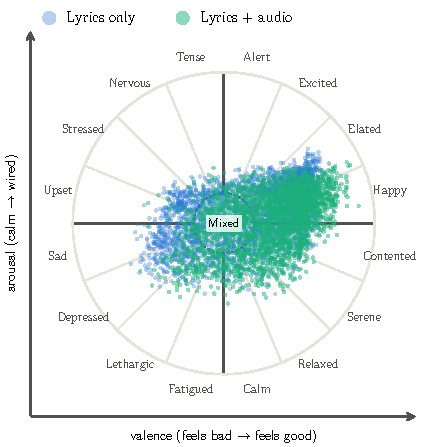
\includegraphics[width=0.93\columnwidth]{figures/catalog_map.pdf}
  \caption{The Senti map. Each dot is one of 5,411 Billboard year-end Hot 100 songs (1960--2025), placed by the blended lyrics + audio score where an Apple Music preview has been scored (2,568 songs) and by lyrics alone otherwise. Sections follow the 16-word circumplex; points within 0.2 of the centre are labelled \emph{Mixed}. The green cloud sits further right than the blue one partly because of the blend and partly because audio-scored songs are mostly from 1960--1989, whose lyrics score happier (Figure~\ref{fig:billboard}).}
  \label{fig:map}
\end{figure}

\section{Related work}

\paragraph{Dimensional music emotion.} The circumplex model~\citep{russell1980circumplex,posner2005circumplex} underlies most continuous MER datasets. DEAM~\citep{aljanaki2017deam} and PMEmo~\citep{zhang2018pmemo} collect valence and arousal ratings from listeners for clips, while MERGE~\citep{louro2024merge} pairs audio with lyrics for about 3,500 songs and derives its labels from AllMusic tags. \citet{kim2010mer} and \citet{yang2012review} survey the field. A recurring finding is that arousal is the easier dimension from audio.

\paragraph{Lyrics and multimodal fusion.} Lyrics features help most on valence, and in some mood categories lyrics alone beat audio~\citep{hu2010lyrics}. Early fusion work combined handcrafted audio descriptors with bag-of-words lyrics~\citep{laurier2008multimodal}. Here the lyrics side is a fine-tuned transformer~\citep{devlin2019bert} compared against RoBERTa~\citep{liu2019roberta} and DeBERTa-v3~\citep{he2023debertav3}. The earlier version of this project was a four-class BERT classifier trained on MoodyLyrics~\citep{cano2017moodylyrics}.

\paragraph{Pretrained audio encoders.} Self-supervised music models such as MERT~\citep{li2024mert} give strong frozen features for downstream tasks; I use a mid-depth MERT layer with a linear head rather than fine-tuning. Whisper~\citep{radford2023whisper} is used only as an analysis tool, to transcribe what is sung in each study preview.

\section{Data}
\label{sec:data}

\paragraph{MERGE.} I use the MERGE lyrics and audio sets (CC BY-NC 4.0). Valence and arousal are rescaled from $[0,1]$ to $[-1,1]$. One fixed split, 80/10/10 stratified by quadrant with seed 42, gives 2,044 training, 256 validation and 256 test songs; it is reused for every model. 1,734 training and 206 test songs also have an audio clip, so all fusion comparisons use those 206 test songs.

\paragraph{Catalogue.} The public map holds the Billboard year-end Hot 100 from 1960 to 2025 (6,601 chart entries from Wikipedia). Genius had usable lyrics for 5,717 entries, or 5,411 unique songs. Lyrics are fetched and scored locally and are never stored or redistributed. For audio, the app looks up each song's 30-second Apple Music preview, preferring the clean edit. 2,568 songs have a stored preview and an audio score. Almost all of them (2,509) are from 1960--1989, because previews were fetched in chart order; the rest of the catalogue is placed by lyrics alone until its previews are scored.

\section{Models}
\label{sec:models}

\begin{figure}[t]
\centering
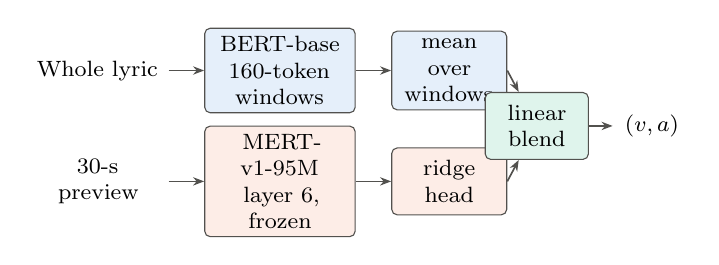
\begin{tikzpicture}[
  font=\footnotesize, node distance=0.35cm and 0.45cm,
  box/.style={draw=ink2, rounded corners=2pt, align=center, inner sep=3pt, minimum height=0.85cm, text width=1.7cm},
  io/.style={align=center, text width=1.55cm},
  arr/.style={-{Stealth[length=4pt]}, ink2, line width=0.6pt}]
  \node[io] (lyr) {Whole lyric};
  \node[box, right=of lyr, fill=lyr!12] (bert) {BERT-base\\160-token windows};
  \node[io, below=0.75cm of lyr] (clip) {30-s preview};
  \node[box, right=of clip, fill=aud!12] (mert) {MERT-v1-95M\\layer 6, frozen};
  \node[box, right=of bert, fill=lyr!12, text width=1.25cm] (tanh) {mean over windows};
  \node[box, right=of mert, fill=aud!12, text width=1.25cm] (ridge) {ridge\\head};
  \node[box, right=0.45cm of $(tanh)!0.5!(ridge)$, fill=fus!14, text width=1.1cm] (blend) {linear\\blend};
  \node[io, right=0.3cm of blend, text width=0.75cm] (out) {$(v,a)$};
  \draw[arr] (lyr) -- (bert); \draw[arr] (bert) -- (tanh);
  \draw[arr] (clip) -- (mert); \draw[arr] (mert) -- (ridge);
  \draw[arr] (tanh.east) -- (blend); \draw[arr] (ridge.east) -- (blend);
  \draw[arr] (blend) -- (out);
\end{tikzpicture}
\caption{Scoring pipeline. Each branch predicts valence and arousal separately; the blend has its own weights per axis, fitted on MERGE validation songs.}
\label{fig:pipeline}
\end{figure}

\paragraph{Lyrics regressor.} \texttt{bert-base-cased}'s pooled output feeds dropout (0.3), a linear layer with two outputs and a $\tanh$, so predictions lie in $[-1,1]$. Training uses the first 160 tokens of each lyric, MSE loss, AdamW at $2\times10^{-5}$ with 10\% linear warm-up, gradient clipping at 1.0, batch size 8 and 5 epochs, keeping the epoch with the best validation MSE. The ``whole-song trained'' variants in Table~\ref{tab:encoders} instead treat every window as its own training example carrying the song's labels, with MSE per window. That did not help (BERT: $-0.012$ valence, $-0.022$ arousal, both within noise), plausibly because a song's overall label is a noisy target for a single verse or outro. At inference a lyric is cut into 160-token windows with stride 120 (at most 8), and the window predictions are averaged. Reading the whole song this way raised test $r$ from 0.70 to 0.72 (valence) and from 0.56 to 0.60 (arousal) compared with the first window alone.

\paragraph{Audio head.} Each clip is cut into 5-second slices with a 2.5-second hop, embedded with MERT-v1-95M~\citep{li2024mert}, and averaged per layer. A ridge regression per axis is trained on the training songs. The encoder (MERT against LAION-CLAP), layer, pooling and regularisation strength were chosen on the validation songs; MERT layer~6 with mean pooling won. Scoring the 2,568 catalogue previews ran on Modal with up to four T4 workers and cost about \$0.11.

\paragraph{Fusion.} The blended score is $\hat y = w_L\,\hat y_L + w_A\,\hat y_A + b$, fitted per axis by least squares on the validation songs with audio rather than the training songs, since the lyrics model has fitted the training lyrics and its training predictions are too good. The fitted weights lean on audio for arousal ($w_L=0.14$, $w_A=1.02$) and use both for valence ($w_L=0.65$, $w_A=0.61$, an audio-to-lyrics ratio of about 0.95). The weights are not constrained to sum to one, and they sum to 1.26 and 1.16. That partly undoes the shrinkage toward the centre that each MSE-trained branch shows (Figure~\ref{fig:merge}).

\paragraph{Statistics.} Differences in Pearson $r$ are tested with a paired bootstrap over songs (2,000 resamples), and I report the percentile 95\% interval. ``Reliably better'' means the interval excludes zero. All correlations are rounded half up from three decimals.

\section{Results on MERGE}
\label{sec:merge}

\paragraph{Lyrics encoders.} Table~\ref{tab:encoders} compares three encoders trained the same way, all read over the whole song. None is reliably better than the deployed BERT on either axis. DeBERTa-v3's valence gain ($+0.027$, CI $[-0.019,+0.075]$) is within noise, and it is reliably worse on arousal ($-0.082$, $[-0.160,-0.007]$). Choosing DeBERTa for valence and BERT for arousal was ruled out because it would select models on the test set. Figure~\ref{fig:merge} shows the deployed model's test predictions, which are pulled toward the centre, most visibly on arousal, where MERGE's labels span a narrow range.

\begin{table}[t]
\centering\footnotesize
\setlength{\tabcolsep}{3pt}
\begin{tabular}{@{}lcccc@{}}
\toprule
& \multicolumn{2}{c}{Valence} & \multicolumn{2}{c}{Arousal}\\
\cmidrule(lr){2-3}\cmidrule(l){4-5}
Encoder & $r$ & MAE & $r$ & MAE \\
\midrule
BERT-base (deployed) & 0.724 & 0.227 & \textbf{0.605} & \textbf{0.180}\\
BERT-base, whole-song trained\,$^*$ & 0.713 & 0.233 & 0.582 & 0.182\\
DeBERTa-v3-base & \textbf{0.751} & \textbf{0.216} & 0.523 & 0.190\\
RoBERTa-base & 0.718 & 0.235 & 0.570 & 0.189\\
Predict the mean & -- & 0.452 & -- & 0.246\\
\bottomrule
\end{tabular}
\caption{Lyrics-only results on the 256 MERGE test songs. The deployed model was trained on the first 160 tokens; the others ($^*$ and the two larger encoders) were trained on all windows. All are read over the whole song.}
\label{tab:encoders}
\end{table}

\begin{figure}[t]
  \centering
  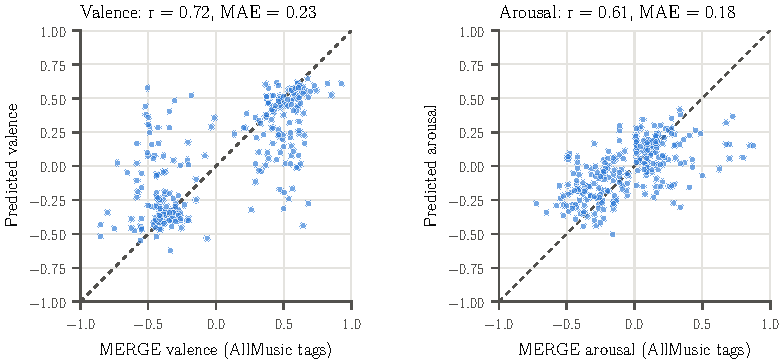
\includegraphics[width=\columnwidth]{figures/merge_scatter.pdf}
  \caption{Deployed lyrics model on the 256 held-out MERGE songs. The dashed line is $y=x$.}
  \label{fig:merge}
\end{figure}

\paragraph{Adding audio.} Table~\ref{tab:fusion} compares the three branches on the 206 test songs that have audio. Audio alone already beats lyrics on arousal (0.75 vs.\ 0.61). The blend is best on both axes, and both gains over lyrics alone are reliable: valence $+0.054$ $[+0.017,+0.095]$, arousal $+0.154$ $[+0.081,+0.235]$. The earlier four-class classifier, mapped to the plane by expected quadrant position, reached only 0.46 and 0.11 on the full test set. That gap is why the map now uses direct regression.

\begin{table}[t]
\centering\footnotesize
\setlength{\tabcolsep}{3.5pt}
\begin{tabular}{@{}lcccc@{}}
\toprule
& \multicolumn{2}{c}{Valence} & \multicolumn{2}{c}{Arousal}\\
\cmidrule(lr){2-3}\cmidrule(l){4-5}
Model & $r$ & MAE & $r$ & MAE\\
\midrule
\textcolor{lyr}{$\blacksquare$} Lyrics (BERT) & 0.716 & 0.223 & 0.611 & 0.162\\
\textcolor{aud}{$\blacksquare$} Audio (MERT L6) & 0.683 & 0.276 & 0.750 & 0.136\\
\textcolor{fus}{$\blacksquare$} Lyrics + audio & \textbf{0.770} & \textbf{0.219} & \textbf{0.765} & \textbf{0.134}\\
\midrule
\multicolumn{5}{@{}l}{\emph{Blend vs.\ lyrics, \dr{} [95\% CI]}}\\
\multicolumn{5}{@{}l}{\quad valence $+0.054$ $[+0.017, +0.095]$}\\
\multicolumn{5}{@{}l}{\quad arousal $+0.154$ $[+0.081, +0.235]$}\\
\bottomrule
\end{tabular}
\caption{Lyrics, audio and fusion on the 206 MERGE test songs with audio.}
\label{tab:fusion}
\end{table}

\section{Listening study}
\label{sec:study}

\paragraph{Song selection.} MERGE's tag-derived labels are not what an app user experiences, so I built an unlisted study page. Its 100 songs were drawn from the catalogue to cover the occupied part of the map evenly. The plane was cut into $0.105\times0.105$ cells, the 100 fullest cells were kept, and each cell contributed one song near its centre, chosen from whichever decade had been picked least so far. This balanced the set across the 1960s--2020s (14--15 songs per decade); without that rule, 86\% of the first draft came from the 1960s. Songs available only as explicit versions, or with profane titles, were replaced by the cell's next candidate. The songs were split into two halves of 50 that each cover the whole map.

\begin{figure*}[t]
  \centering
  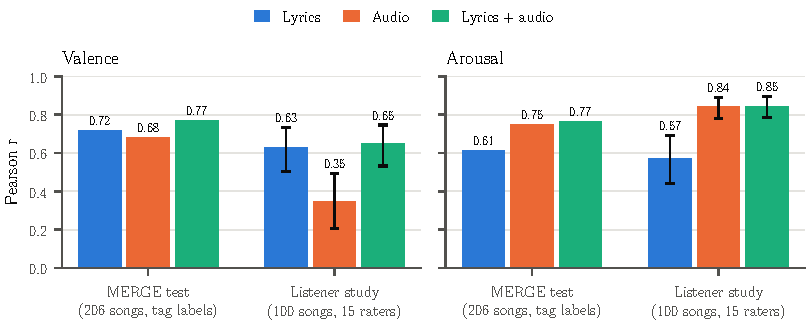
\includegraphics[width=0.78\textwidth]{figures/r_bars.pdf}
  \caption{Pearson $r$ of each branch with MERGE's tag-derived labels (left group of each panel) and with the median listener placement in the study (right group). Error bars are 95\% bootstrap intervals over the 100 study songs.}
  \label{fig:rbars}
\end{figure*}

\paragraph{Procedure.} After two unscored warm-up songs, each rater heard one half, the half fewer people had finished, in their own random order. Four hidden repeats were spread through the second half, each at least 10 songs after its first play and never an instrumental. For each clip the rater dragged a point on a plain grid with no emotion words, labelled only at the edges: negative to positive mood and calm to energetic. The instructions asked for ``the mood the song puts across, not how it makes you feel.'' The \emph{Next} button unlocked after 8 seconds of listening. Raters could also mark a song as known, say a clip had no singing, or skip it. Age range and gender were optional and are not analysed here. Raters gave consent on the first screen; answers are stored under random rater codes, and payment codes are kept apart from the answers so that the two cannot be linked. Raters were recruited through personal networks; ten paid places were offered, along with an unpaid link.

\paragraph{Analysis set.} The export holds 548 rows from 15 raters: 438 first-listen placements of the 100 study songs, 37 hidden repeats, 4 skips, and 69 placements of songs from an earlier draft of the list, heard by three early raters, which are excluded. For each song the listener answer is the median of first-listen placements; every song has at least 3 raters (median 4, at most 6). All three model scores are compared on these same 100 songs. Median listening time was 9 seconds per clip. On the 37 hidden repeats, a rater's second placement correlates with their first at $r=0.73$ for valence and $0.70$ for arousal, which gives a rough ceiling for agreement with a single listener. Eight raters placed a full half of about 50 songs; the other seven placed between 1 and 11.

\section{Results against listeners}
\label{sec:listeners}


\paragraph{Correlation.} Figure~\ref{fig:rbars} puts the two evaluations side by side. On arousal the model holds up at least as well with real listeners as on MERGE. The blend reaches $r=0.85$ $[0.79,0.89]$, and its gain over lyrics alone is larger than on MERGE: $+0.28$ $[+0.17,+0.39]$, against $+0.15$. On valence the blend scores $0.65$ $[0.53,0.75]$, about the same as lyrics alone ($+0.02$, $[-0.04,+0.08]$). Almost all of the drop from MERGE comes from the audio branch, which falls from 0.68 to 0.35. The two evaluations are not strictly like for like: the study songs were picked to cover the map evenly, which tends to raise $r$, especially on arousal, and MERGE's labels and the listeners' are different kinds of ground truth. Figure~\ref{fig:studyscatter} shows the song-level picture; the model's arousal range is narrower than listeners', so MAE (0.28 for the blend) is worse than the correlation suggests. The blend's scale is matched to MERGE's labels, which are themselves compressed, likely because each song's score averages several mood tags, while listeners use the whole grid. The predictions are well ordered but squeezed toward the centre relative to people.

\begin{figure}[t]
  \centering
  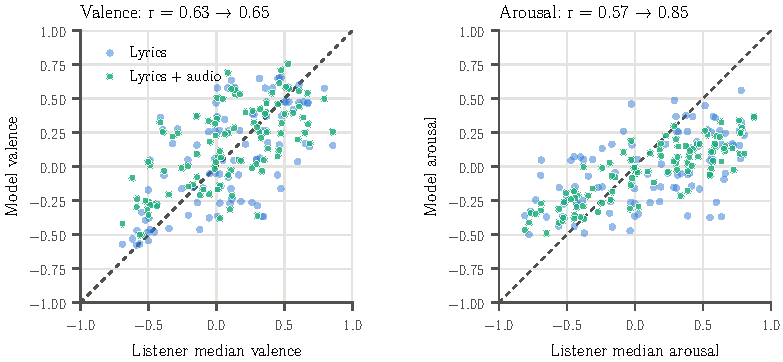
\includegraphics[width=\columnwidth]{figures/study_scatter.pdf}
  \caption{Model score against median listener placement for the 100 study songs: lyrics alone (blue) and the deployed blend (green).}
  \label{fig:studyscatter}
\end{figure}

\subsection{Is the model as good as a person?}
\label{sec:crowd}

Correlation with a crowd median favours the model unfairly if a single rater is then compared with a median that includes that rater's own answer. I therefore measure everyone against the same leave-one-out target. For each placement, the target is the mean placement of that song by all \emph{other} raters. I use the mean rather than the median here because a song has a median of 4 raters, which leaves 2--5 others, and with so few the mean is smoother (for 2 the two are equal). The leave-one-out median gives the same ordering: the average rater is 0.53 from it, the blend 0.43, and the blend beats 11 of 15 raters. Each rater's distance to that target is compared with each model's distance to it, over the same 438 placements. Including raters in their own consensus would have made people look about 20\% better than they are (0.40 instead of 0.50).

\begin{figure}[t]
  \centering
  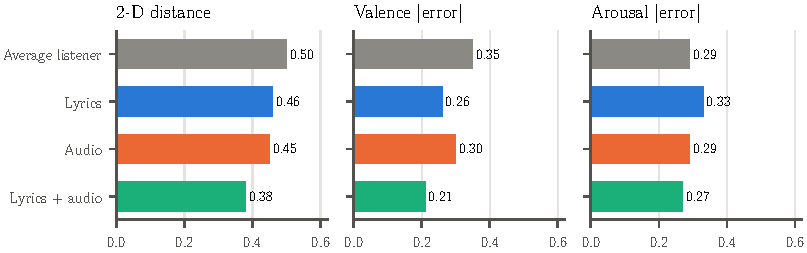
\includegraphics[width=\columnwidth]{figures/consensus_distance.pdf}
  \caption{Mean distance from the leave-one-out consensus over 438 first-listen placements. Lower is better.}
  \label{fig:consensus}
\end{figure}

Figure~\ref{fig:consensus} shows that the blend lands closer to the consensus than the average rater does: 0.38 against 0.50 in 2-D distance, about 24\% closer. Person by person, the blend is closer than 12 of the 15 raters, while lyrics alone and audio alone each beat 9. The seven raters who placed only 1--11 songs have noisy averages. Of the 8 raters who placed about 50 songs each, the blend beats 6, ties one (0.41) and trails one (0.39 vs.\ 0.42). Most of the advantage is on valence, where the blend's error (0.21) is well under the average person's (0.35). On arousal, people are already about as close to each other as the audio model is.

\subsection{Where does listener valence come from?}
\label{sec:valence}

The weak audio valence score raises a question. Do listeners judge valence by the sound, which the audio head fails to capture, or by the words? People hear a median of 9 seconds, often before any singing, which argues for the sound. Three tests bear on it.

\paragraph{Disagreement songs.} On 31 of the 100 songs, the lyrics and audio valence scores are at least 0.4 apart. Listeners sided with the lyrics on 22 of them and with the audio on 9. The audio wins are mostly sad or ambivalent lyrics over upbeat pop. In \emph{Feel It Still} (Portugal.\ The Man), for example, lyrics score $-0.16$, audio $+0.56$ and listeners $+0.47$. That is the pattern a ``people hear the sound'' account predicts. The lyrics wins look more like the audio head misreading the clip. In \emph{Unfaithful} (Rihanna), audio scores $+0.42$ while listeners place it at $-0.62$, close to the lyrics' $-0.53$. On arousal, listeners sided with audio on 6 of the 7 disagreements.

\paragraph{What is actually in the preview.} Whisper~\citep{radford2023whisper} (\texttt{medium}), run on Modal for about \$0.07, transcribed all 100 study previews. In 38 of them nothing is sung in the first 9 seconds, and in 39 less than 3 seconds of singing falls there. On those 39 songs, the lyrics model matches listener valence less well ($r=0.56$, against 0.68 for the 61 clips with singing), and adding audio helps more (0.56 to 0.63, against no change). I then scored only the words transcribed from each clip with the same BERT model; 68 clips had transcribable words. Table~\ref{tab:preview} shows the result. Preview-only lyrics are reliably \emph{worse} than whole-song lyrics for valence ($-0.16$, $[-0.32,-0.01]$), and in a leave-one-song-out cross-validated blend they add nothing to the whole-song score. For arousal the two are equal.

\begin{table}[t]
\centering\footnotesize
\setlength{\tabcolsep}{4pt}
\begin{tabular}{@{}lcccc@{}}
\toprule
$r$ with listeners & Whole lyric & Preview lyric & Audio & Blend\\
\midrule
Valence & \textbf{0.69} & 0.53 & 0.39 & 0.67\\
Arousal & 0.60 & 0.61 & 0.83 & \textbf{0.84}\\
\bottomrule
\end{tabular}
\caption{The 68 study songs whose preview contains transcribable singing. ``Preview lyric'' scores only the words Whisper heard in the clip.}
\label{tab:preview}
\end{table}

So, even after hearing about 9 seconds, listeners' valence matches what the whole song is about better than the words they actually heard. Familiarity does not explain it: individual placements of songs the rater marked as known (35) track the lyrics score no better than the rest (0.42 vs.\ 0.44), and raters who listened for less than the median 9 seconds were no less lyric-aligned than those who listened longer (0.53 vs.\ 0.50). My reading, which these data suggest but do not prove, is that the whole-lyric score also captures a song's overall character, which comes through in its key, voice and production. Two caveats apply. Whisper mishears some sung words, and the lyrics model was trained on full lyrics, not short fragments.

\paragraph{The valence fusion weight.} The MERGE-fitted blend gives audio about 0.95 times the weight of lyrics. Refitting on the study songs with leave-one-out cross-validation roughly halves that: lyrics 0.60, audio 0.33, giving $r=0.63$ against 0.61 for lyrics alone. Figure~\ref{fig:weight} shows why that is not grounds for a change. Correlation is nearly flat across a wide range of weights: 0.63 with no audio, 0.66 at a ratio of 0.5, 0.65 at the current 0.95, and 0.62 at 1.5. The bootstrap interval for the best ratio runs from about 0.15 to 1.1, which includes the current weight. Moving to 0.5 changes $r$ by $+0.01$ $[-0.02,+0.03]$. In a split-half check, fitting on one half picks 0.85 and fitting on the other picks 0.35, and neither beats the current weight on the half it was not fitted on. The deployed weight therefore stays. A rough power estimate says that settling the question needs about 300 rated songs, and new songs help more than repeat ratings of the same ones.

\begin{figure}[t]
  \centering
  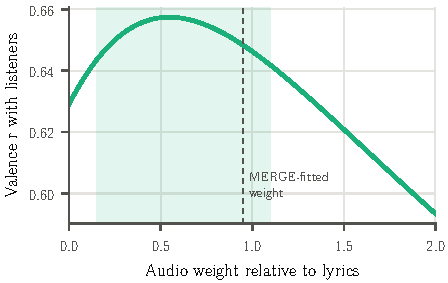
\includegraphics[width=0.82\columnwidth]{figures/valence_weight.pdf}
  \caption{Valence correlation with listeners as the audio-to-lyrics weight ratio varies. The shaded band is the 95\% bootstrap interval for the best ratio; the dashed line is the MERGE-fitted ratio used in the app.}
  \label{fig:weight}
\end{figure}

\section{An application: six decades of hits}

With every song scored, the catalogue can be read in aggregate. Figure~\ref{fig:billboard} plots the mean lyrics-model score of each year's Billboard hits. Predicted valence falls from about 0.19 in the early 1960s to about 0.08 in the early 2020s, and predicted arousal rises from about $-0.05$ to $+0.04$. These are model predictions, not listener ratings, and the model's own correlation with listeners is 0.63 and 0.57 on these axes. They use the lyrics branch alone, because audio coverage is concentrated before 1990. They are best read as a demonstration of what the map supports, not as a cultural finding.

\begin{figure}[t]
  \centering
  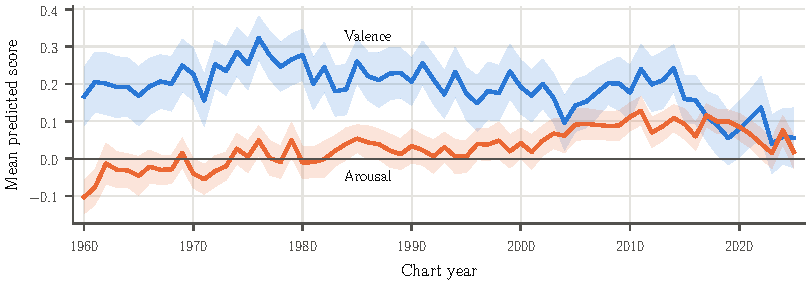
\includegraphics[width=\columnwidth]{figures/billboard_trend.pdf}
  \caption{Mean predicted valence and arousal of Billboard year-end Hot 100 songs by year (lyrics model, 5,411 unique songs). Bands are $\pm1.96$ standard errors of the yearly mean of predictions.}
  \label{fig:billboard}
\end{figure}

\section{Limitations}

\begin{itemize}\setlength\itemsep{0.15em}
  \item \textbf{Small study.} 100 songs and 15 raters, of whom 8 placed about 50 songs each. Intervals are wide, and the study cannot separate valence weights that differ by a factor of two. Three early raters heard a first draft of the song list; their placements of songs outside the final list are excluded.
  \item \textbf{Convenience sample.} Raters were recruited through personal networks, and catalogue songs are mostly older US hits. Neither represents all listeners or all music.
  \item \textbf{Proxy labels.} The models are trained only on MERGE's tag-derived labels. The audio head may have learned how AllMusic taggers describe a sound rather than what listeners hear in a preview.
  \item \textbf{Clip mismatch.} Apple previews are often a different part of the song than MERGE's clips. That may explain part of the audio valence drop.
  \item \textbf{Frozen audio features.} The audio branch is a linear head on a frozen encoder. Fine-tuning end to end is the obvious next experiment.
  \item \textbf{Lyrics only in English.} Songs without lyrics on Genius (instrumentals and some older or non-English songs) are missing from the catalogue.
\end{itemize}

\section{Conclusion}

A simple late fusion of a lyrics transformer and frozen music embeddings places songs on the circumplex well enough that, for the songs in this study, it agrees with a crowd of listeners more closely than most individual listeners do. The two modalities divide the work cleanly. Audio carries arousal, and the evidence points to the song's overall meaning, rather than the few words heard, as the carrier of valence. The listening study changed the picture that MERGE alone gave: arousal held up better with people than on tag labels, and audio valence held up much worse. Evaluating against the actual user experience is cheap and worth doing. Next steps are a second study round aimed at the songs where the model is least sure, to settle the valence weight with about 300 songs; fine-tuning the audio encoder end to end on MERGE; and an ``explain this song'' view that shows how much of each placement comes from lyrics and how much from audio.

\paragraph{Data and code.} Code, score files (no lyrics) and the analysis scripts are at \url{https://github.com/jason-d-garcia/senti}. MERGE annotations are redistributed under CC BY-NC 4.0, with values rescaled. Lyrics are never stored or published.

\small
\bibliographystyle{abbrvnat}
\bibliography{refs}

\end{document}
